\chapter{Common solutions}
In this chapter we will try to summarize the most common technics for solving the rendering equation in the presence of participating media. Many methods are used today and it's way beyond the scope of this thesis to do a proper summary of them, so only widely used methods related to the context of this thesis were picked.
\section{ Rasterization}
Rather than talking about game solutions, where is the main goal to render everything real time and physical accuracy of lighting is less important than plausible smooth graphics, we will have a look on rasterization used in offline rendering.
\\
\\
Rasterization comes as a nature choice, when it comes to particle rendering. It's key benefit is that the whole scene geometry doesn't have to fit into the RAM \footnote{Computer main random access memory.}, in the cost of linear rendering complexity. Because list of primitives, be it points, lines or triangles, is rasterized one by one in the frame-buffer.

\begin{minipage}{\linewidth}
      \begin{minipage}{0.45\linewidth}
          \begin{figure}[H]
              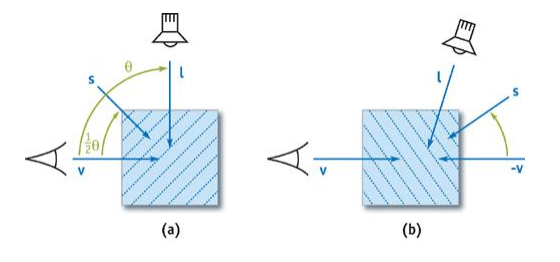
\includegraphics[width=\linewidth]{images/halfanglenvidia.png}
              \captionsetup{width=\linewidth}
              \caption[Half axis angle particle sorting and rendering.]{Illustration of the half axis angle determination for single particle sorting pass. Source \cite{NVIDIA}.}\label{fig:HAA}
          \end{figure}
      \end{minipage}
      \hspace{0.05\linewidth}
      \begin{minipage}{0.45\linewidth}
          \begin{figure}[H]
              \includegraphics[width=\linewidth]{\cestaImg nvidiasmokeparticles.jpg}
              \captionsetup{width=\linewidth}
              \caption[Nvidia smoke particle demo. Source \cite{NVIDIA}.]{This image has been rendered using multiple shadow maps for particle direct illumination on gpu. Source \cite{NVIDIA}.}\label{fig:NVS}
          \end{figure}
      \end{minipage}
  \end{minipage}
  \\
  \\
 \noindent{
Almost all the algorithms widely used rely on the same kind of preprocessing stage. The particles should be ideally sorted from the furtherest to the closest, and rasterized in this order, so that the alpha blending works correctly. Which is quite costly, considering we should sort millions of particles twice. Once for the camera view and once for the shadow map generation light view. To overcome this issue a half-angle axis sorting can be used, where we sort particles along a half angle axis between the camera and the light only once as can be seen on fig. \ref{fig:HAA}.
}
\\
\\
Also shadow map containing only a nearest depth is practically useless when used with millions of partially transparent particles. To cope with this we can either rasterize the particles in the common layer batches for camera view and light view to sample progressively reducing transmittance as used in nVidia demo fig. \ref{fig:NVS}. 
\\
\\
Or we can eventually use deep shadow maps \cite{LokDSM}, where is the occlusion function of depth\footnote{The function is usually represented as lookup table containing [depth,transmittance] tuples.} instead of a single value per pixel in the case of regular shadow maps. This approach allows pre-filtering\footnote{Object can occlude only partial part of the pixel, thus adding only appropriate amount of occlusion in incident depth.} which leads to suppression of both depth and aliasing artifacts commonly seen in shadow map renderings.
\\
\clearpage{}
\noindent{
Even tough only single scattering volume interaction can be modeled this way, it's very popular method widely used in the VFX industry, because it can handle very efficiently even billions of particles as can be seen on fig. \ref{fig:KRAK}. 
}

\myFigure{0.95}{\cestaImg krakatoa.jpg}{Krakatoa particle and volume rendering.}{Examples of rasterization Krakatoa particle render used in feature film productions \cite{KRAK} .}{fig:KRAK}

\section{Raytracing}
Another very popular method for solving rendering equation is raytracing. Which is way more flexible than rasterization, in the terms of complex light scene interaction. The flexibility unfortunately goes in hand with an additional cost of acceleration structure build and usage for a ray primitive intersection.

% great page for latex equation typing http://www.codecogs.com/latex/eqneditor.php
Quasi Monte Carlo equation
\begin{equation*}
\int _{I^{S}}f(x)dx\approx\frac{1}{N}\sum_{i=1}^{N}f(x_{i})),
\end{equation*}
%\int _{I^{S}}f(x)dx\approx\frac{1}{N}\sum_{i=1}^{N}f(x_{i})),

\subsection{Raymarching volumes}
The key aspect of raytracing volumes is the transmittance computation.

More recently, another technique has become popular for sampling distances along a ray in an inhomogeneous medium. The idea comes from the neutron transport community in the 60s and has various names (delta tracking, pseudo-scattering); we’ll call it Woodcock tracking in effort to promote original paper.

pbrt single scattering
can support procedural volumes and any type of lighting

\subsection{Unbiased methods}

\myFigure{0.55}{\cestaImg temp.jpg}{Unbiased raytracing methods.}{Examples of unbiased raytracing methods, from left \ita{path tracing, light tracing, bidirectional path tracing}. The principle is pictured on the top raw and example renderings are in the bottom one.}{fig:UNBRT}

Path tracing, light tracing fig. \ref{fig:UNBRT}
Plus and cons - very slow no caching recomputation of visibility factor

\subsection{Biased methods}

\cite{jarosz08thesis} %jarosz thesis irradiance caching
irradiance caching, Photon tracing, final gather ...
Plus and cons

